%
% Annual Cognitive Science Conference
% Sample LaTeX Paper -- Proceedings Format
%

% Original : Ashwin Ram (ashwin@cc.gatech.edu)       04/01/1994
% Modified : Johanna Moore (jmoore@cs.pitt.edu)      03/17/1995
% Modified : David Noelle (noelle@ucsd.edu)          03/15/1996
% Modified : Pat Langley (langley@cs.stanford.edu)   01/26/1997
% Latex2e corrections by Ramin Charles Nakisa        01/28/1997
% Modified : Tina Eliassi-Rad (eliassi@cs.wisc.edu)  01/31/1998
% Modified : Trisha Yannuzzi (trisha@ircs.upenn.edu) 12/28/1999 (in process)
% Modified : Mary Ellen Foster (M.E.Foster@ed.ac.uk) 12/11/2000
% Modified : Ken Forbus                              01/23/2004
% Modified : Eli M. Silk (esilk@pitt.edu)            05/24/2005
% Modified : Niels Taatgen (taatgen@cmu.edu)         10/24/2006
% Modified : David Noelle (dnoelle@ucmerced.edu)     11/19/2014
% Modified : Roger Levy (rplevy@mit.edu)     12/31/2018



%% Change "letterpaper" in the following line to "a4paper" if you must.

\documentclass[10pt,letterpaper]{article}

\usepackage{cogsci}

\cogscifinalcopy % Uncomment this line for the final submission

\usepackage{graphicx}
\usepackage{pslatex}
\usepackage{apacite}
\usepackage{float} % Roger Levy added this and changed figure/table
                   % placement to [H] for conformity to Word template,
                   % though floating tables and figures to top is
                   % still generally recommended!

%\usepackage[none]{hyphenat} % Sometimes it can be useful to turn off
%hyphenation for purposes such as spell checking of the resulting
%PDF.  Uncomment this block to turn off hyphenation.


\setlength\titlebox{8.5cm}
% You can expand the titlebox if you need extra space
% to show all the authors. Please do not make the titlebox
% smaller than 4.5cm (the original size).
%%If you do, we reserve the right to require you to change it back in
%%the camera-ready version, which could interfere with the timely
%%appearance of your paper in the Proceedings.



\title{Controlling the retrieval of general vs specific semantic knowledge in the instance theory of semantic memory}

\author{{\large \bf Matthew J. C. Crump (mcrump@brooklyn.cuny.edu)} \\
  Department of Psychology, 2900 Bedford Ave \\
  Brooklyn, NY 1120 USA
  \AND {\large \bf Randall K. Jamieson (randy.jamieson@umanitoba.ca)} \\
  Department of Psychology, 190 Dysart Rd \\
  Winnipeg, MB R3T 2N2 Canada
  \AND {\large \bf Brendan T. Johns (brendan.johns@mcgill.ca)} \\
  Department of Psychology, 2001 McGill College Ave \\
  Montreal, QB H3A 1G1 Canada
  \AND {\large \bf Michael N. Jones (jonesmn@indiana.edu)} \\
  Department of Psychological and Brain Sciences, 1101 E. 10th St. \\
  Bloomington, IN 47405 USA}


\begin{document}

\maketitle


\begin{abstract}
Distributional models of semantic cognition commonly make simplifying assumptions, such as representing word co-occurrence structure by prototype-like high-dimensional semantic vectors, and limit how retrieval processes may contribute to the construction and use of semantic knowledge. More recently, the instance theory of semantics \cite<ITS, >{jamiesonInstanceTheorySemantic2018a} reconceived a distributional model in terms of instance-based memory, allowing context-specific construction of semantic knowledge at the time of retrieval. By simulation, we show that additional encoding and retrieval operations, consistent with learning and memory theory, can play a crucial role in flexibly controlling the construction of general versus specific semantic knowledge. We argue this consolidation of processing principles holds insight for distributional theories of semantic cognition.

\textbf{Keywords:}
distributional semantics; higher-order similarity; instance theory; surprise-driven learning; retrieval
\end{abstract}

\section{Introduction}\label{introduction}

People flexibly understand word meaning at multiple levels of similarity and in different contexts. For example, the word cat could be similar to subordinate (tiger), basic (dog) or superordinate (animal) category words; associates (house, hat, or Felix); alternative meanings (a person in jazz, or Caterpillar machinery); or words in general compared to nonwords. How people flexibly control the specificity of their semantic knowledge remains unclear. Stable semantic representations for words may become positioned in high-dimensional semantic space to permit multiple comparisons for meaning along general and specific lines. Or, semantic representations could be more labile, potentially granting processes associated with encoding and retrieval operations control over the construction of general versus specific semantic meaning. The present work merges assumptions from three memory models, MINERVA 2 \cite{hintzmanMINERVASimulationModel1984},  the instance theory of semantics \cite<ITS,>{jamiesonInstanceTheorySemantic2018a} and the instance theory of associative learning \cite<MINERVA-AL,>{jamiesonInstanceTheoryAssociative2012}, to examine how learning and memory operations participate in the flexible construction of general and specific semantic knowledge.

As accounts of semantic cognition, we distinguish between representation and retrieval models. Distributional models typically articulate processes for forming semantic representations but underspecify the role of retrieval. For example, models like LSA \cite{landauerSolutionPlatoProblem1997}, BEAGLE \cite{jonesRepresentingWordMeaning2007}, and word2vec \cite{mikolovDistributedRepresentationsWords2013} represent word meaning in terms of high-dimensional vectors sensitive to co-occurrence structure in natural text, whereby words closer in semantic space are closer in meaning. Furthermore, representations are prototypic because each word has one vector that roughly averages over co-occurrence structure with other words in the corpus. The prototype assumption is obvious for polysemous words. For example, ``bank'' could refer to a river or financial institution; but, a prototype representation averages the distinction with a single vector partway between the two meanings. Nevertheless, prototype representations can be sensitive to multiple levels of similarity (e.g., cat can be similar to lion and animal) because words can be positioned in high-dimensional space to somewhat align with multiple levels of meaning. Retrieval minimally involves comparing word similarity in high-dimensional space, but does not interact with encoding or construction of semantic representations. Finally, models use various pre-processing steps, like stop-word exclusion, log and entropy transformations (LSA), and negative information sub-sampling (word2vec), or post-processing transformations of base-rate information \cite<e.g., >{johnsRoleNegativeInformation2019} to further improve the specificity of semantic representations.

Outside of semantic modeling, instance/exemplar theories have risen against prototype accounts \cite<e.g., in categorization and concept formation, >{jacobyNonanalyticCognitionMemory1984}. Instance theory assumes that memory encodes a history of richly featured examples as traces, and retrieves them in context-specific fashion by their similarity to patterns in the immediate environment. Although the composition of examples in memory is stable, knowledge as content retrieved from memory is labile depending on retrieval conditions and operations.

Recently, ITS \cite{jamiesonInstanceTheoryAssociative2012} applied instance theory to distributional semantics by combining BEAGLE word representations \cite{jonesRepresentingWordMeaning2007} with MINERVA 2 encoding and retrieval operations \cite{hintzmanMINERVASimulationModel1984}. In BEAGLE, a semantic vector is a prototype aggregating over sentence representations containing a word. By contrast, ITS encodes individual sentences as memory traces, and aggregates over them at retrieval allowing retrieval conditions to selectively modulate the construction of word meaning. For example, ITS handles polysemy by retrieving the meaning of a probe word (bank) depending on the conditions of local context (river vs. piggy). ITS showed how the selective construction of semantic knowledge from memory can depend on retrieval \emph{conditions} (e.g., probe context), but did not fully consider how its encoding and retrieval \emph{operations} offer additional control over the specificity of semantic representations.

Here, we establish the value of importing assumptions about encoding and retrieval operations from learning and memory theory into a modification of ITS (ITS 2). A parsimonious feature of ITS 2 is the consolidation of processing assumptions made between variants of MINERVA 2 that were not originally expressed in ITS. For example, MINERVA-AL \cite{jamiesonInstanceTheoryAssociative2012} is an instance account of associative learning phenomena that employed a modified encoding rule, termed \emph{discrepancy encoding}. Whereas MINERVA 2 and ITS encode each new experience as a raw trace in memory, MINERVA-AL mimicked the principle of surprise-driven learning \cite{rescorlaTheoryPavlovianConditioning1972} by encoding only features of a new experience that were unexpected by memory. In ITS 2, we show that a form of \emph{discrepancy encoding}, termed \emph{weighted expectancy subtraction} (because it can be performed at encoding or retrieval) controls the specificity of semantic knowledge. Similarly, MINERVA 2 allowed the possibility of \emph{iterative retrieval}, where memory responses inspire successive waves of retrieval. We show that iterative retrieval in ITS 2 allows traversal of higher orders of semantic similarity and controls the generality of semantic knowledge. In the general discussion, we speculate that encoding and retrieval operations are crucial for negotiating the integration of general and specific expectations for word co-occurrence in semantic representations, and may approximate post-processing transforms for weighting word base rate information known to improve word-embedding quality \cite{johnsRoleNegativeInformation2019}.

\subsection{ITS and ITS 2}

We first define ITS and ITS 2, and then trained them on an artificial language with known word co-occurrence structure. This enabled clear accounting of encoding and retrieval operations controlled recovery of specific and general aspects of the semantic space.

\subsubsection{Word representation}

Following BEAGLE, words are arbitrary perceptual objects with no pre-existing similarity. Each word, is assigned an environment vector, $e_i$, by randomly sampling \(n\) values from a normal distribution (\(\mu = 0\), \(\sigma = 1/\sqrt{n}\)), where \(n\) determines the dimensionality of the vector space. Thus, all words are ortho-normal in expectation. ITS can accommodate other representational assumptions and we used a identity matrix, with the diagonal set to 1, and the number of rows/columns equal to the number of words in the language. We used a one-hot coding scheme for pedagogical reasons, and the results of the following simulations do not depend on this coding scheme.

\subsubsection{Memory}

ITS preserves experiences with individual sentences in memory. For example, committing a sentence to memory involves summing the environmental vectors for the words in the sentence, and entering the composite vector as a new row in the matrix:

\begin{equation}
M_i = c_i = \sum_{j=1}^{j=h} e_{ij}
\label{eq:memory}
\end{equation}

\noindent \(M\) is the memory matrix, and \(c_i\) is a sentence context. \(c_i\) is stored in a new row in \(M_i\) as a composite trace by summing the \(e_{ij}\) environment vectors for each word, from \(1\), to \(h\), in the sentence. For example, the sentence context, $c_i$, ``I like cats'' is the sum of \(e_{I} + e_{like} + e_{cats}\) word environment vectors. The number of words inside a trace, $h$, is a windowing parameter that must be larger than one word, otherwise the memory will return perceptually similar traces, rather than semantically similar ones. We note that the memory matrix becomes a document-term matrix of word frequencies when the environment vectors for words are taken from an identity matrix.

\subsubsection{Retrieval}\label{retrieval}

Word meaning is constructed at retrieval. Memory is probed with a word and returns an echo response. The echo is the sum of similarity weighted traces to the probe, and taken as the semantic vector for the probe word. Retrieval and echo construction follow MINERVA 2. First, memory \(M\) is probed, $p$, with a word environment vector ($p_j = e_i$) and the cosine similarities between \(p_j\) and all traces \(M\) are computed to produce a vector of trace activations \(a_i\):

\begin{equation}
a_i = (\frac{\sum_{j=1}^{j=n}p_j \times M_{ij}}{\sqrt{\sum_{j=1}^{j=n}p_j^2}\sqrt{\sum_{j=1}^{j=n}M_{ij}^2}})^{\tau}
\label{eq:activation}
\end{equation}

\noindent where, \(a_i\) is the activation (cosine similarity to probe) of trace \(i\) in memory, \(p_j\) are the \(jth\) features of the probe, \(M_{ij}\) are the \(jth\) features of each trace \(i\) in memory, and \(n\) is the number of columns in memory setting the dimensionality of the vector space. The vector of activations is raised to a power, \({\tau}\), controlling a retrieval gradient determining selectivity in the composition of the echo. The activation vector is a record of similarity between the traces and the probe spanning the range \(-1\) to \(1\), with \(a_i = 1\) when a trace is identical to the probe, \(a_i = 0\) when a trace is orthogonal to the probe, and \(a_i = -1\) when the trace is opposite the probe. When  \({\tau} = 0\), activations are squashed to -1 or 1. When \({\tau}\) is an even number, the original sign of each activation value is retained after multiplication. 

Second, the memory-based semantic representation, $sem_i$, for the probe word is retrieved as an echo by summing the traces in proportion to their activation. Specifically, all traces in memory are multiplied by their activations, and the echo is formed by summing the weighted traces:

\begin{equation}
sem_i = echo_j = \sum_{i=1}^{i=m}\sum_{j=1}^{j=n}a_i \times M_{ij}
\label{eq:echo}
\end{equation}

\noindent where, \(echo_j\) is the \(jth\) feature of the echo, \(m\) is the number of traces in memory, \(a_i\) is the activation of trace \(i\), and \(M_{ij}\) are the \(jth\) values of each trace \(i\) in memory. In ITS, the echo vector is used as the semantic representation for the probe word, $sem_i$.

Words are compared for semantic similarity by comparing their respective echoes. Semantic similarity between two probes words, $cos(p_1,p_2)$, is computed between their respective echoes using a cosine.

\begin{equation}
cos(p_1,p_2) = \frac{\sum_{j=1}^{j=n}echo_{1j} \times{} echo_{2j}}{\sqrt{\sum_{j=1}^{j=n}echo_{1j}^2}\sqrt{\sum_{j=1}^{j=n}echo_{2j}^2}}
\label{eq:semanticsim}
\end{equation}

Briefly, words become similar to one another by appearing in similar sentences. For example, probing the word ``doctor'' will return an echo comprised of a sum over sentences including ``doctor''. This echo will be similar to the echo for words like ``nurse'' which sums over sentences with overlapping words (e.g., hospital).

\subsection{ITS 2: Weighted expectancy subtraction at encoding}

ITS 2 implements \emph{weighted expectancy subtraction} during encoding in a similar manner to MINERVA-AL's \emph{discrepancy encoding} rule. The difference is the subtraction between the probe and the echo is weighted by \(x\), controlling the amount of expectation to be subtracted. Weighted expectancy subtraction is applied at each step across training. For example, when a new sentence is experienced, the sentence context vector \(c_i\) is used as a probe to memory to generate an echo. The echo represents the memories' expectation for the new sentence. If the new sentence is fully expected, then the memory can reconstruct the new sentence on the basis of its existing traces. The magnitude of the echo vector contains the sum of many traces, and is generally much larger than the magnitude of the sentence context vector. As a result, before subtraction, the probe and echo vectors are normalized,

\begin{equation}
c'_j = \frac{c_j}{\max | c_{j,n} |}
\label{eq:normprobe}
\end{equation}

\noindent where, \(c_j\) is a sentence context probe vector, and the elements of \(c_j\) are divided by the largest absolute value in \(c_j\), to produce the normalized \(c'_j\). Similarly, the echo is normalized such that,

\begin{equation}
echo'_j = \frac{echo_j}{\max | echo_{j,n} |}
\label{eq:normecho}
\end{equation}

\noindent where, \(echo_j\) is an echo vector, and the elements of \(echo_j\) are divided by the largest absolute value in \(echo_j\), to produce the normalized \(echo'_j\).

Next, the new trace encoded to memory is defined by subtraction of a weighted normalized echo from the normalized probe,

\begin{equation}
M_{ij} = c'_j  - x \cdot echo'_j
\label{eq:ITS2encoding}
\end{equation}

\noindent where, \(M_{ij}\) is the new row entry in the memory matrix, and \(x\) is a weighting parameter (from 0 to 1), controlling how the proportion of the normalized echo subtracted from the normalized probe. When \(x\) is set to 0, ITS 2 becomes equivalent to ITS.

\subsection{ITS 2: Weighted expectancy subtraction at retrieval}

ITS 2 can conduct \emph{weighted expectancy subtraction} at retrieval, after training is complete. Memory is constructed identically to ITS, except weighted expectancy subtraction occurs at retrieval through a two-step \emph{iterative retrieval} process. A probe word generates an echo from memory, and the echo is submitted as an ``internal'' probe to generate a second echo. The semantic representation for the word is taken as a weighted subtraction of the normalized second echo from the normalized first echo.

The first echo, \(echo_\alpha\), is generated in the usual way, but then resubmitted as a probe to construct a second echo, \(echo_\beta\), by the same equations \ref{eq:activation} and \ref{eq:echo} used to construct \(echo_\alpha\). Both \(echo_\alpha\) and \(echo_\beta\) are normalized following equation \ref{eq:normecho}. The semantic representation for a word, $sem_i$, with weighted expectancy subtraction at retrieval in ITS 2 is:

\begin{equation}
sem_i = echo'_\alpha - x \cdot echo'_\beta
\label{eq:ITS2retrieval}
\end{equation}

\noindent where, \(sem_i\) is the semantic representation for the \(ith\) word, and \(x\) is a weighting parameter varying from 0 to 1 controlling the proportion of \(echo'_\beta\) subtracted from \(echo'_\alpha\).

\section{Simulations}

\begin{figure*}

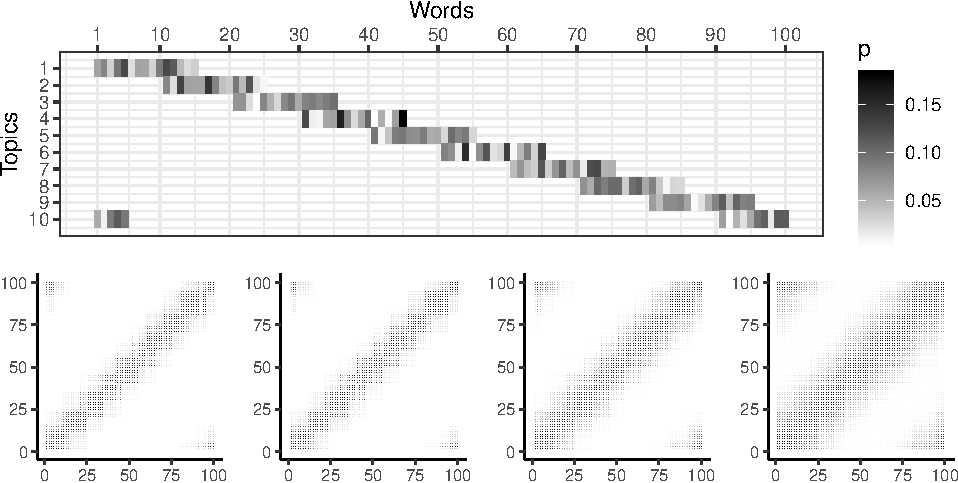
\includegraphics[width=\textwidth]{ITS_cogsci_files/figure-latex/artlang-1.pdf}

\caption{Upper: The topic-word probability matrix defining the artificial language. Darker colors represent higher probability of word occurrence. Lower: Word-word similarity matrices from the first to fourth order.}\label{fig:artlang}
\end{figure*}

Our aim was to characterize how ITS and ITS 2 recover specific and general aspects of semantics from co-occurrence. First, we created an artificial language with known co-occurrence structure. Next, we trained ITS on sentences from the artificial language and compared the semantic structure of ITS vectors to direct measures of the semantic structure of the language. We were interested in determining which aspects of the language ITS recovers by default. Last, we show that encoding and retrieval operations in ITS 2 provide control over the specificity of semantic knowledge production.

\subsection{Artificial language}

The artificial language contained no grammar and only semantic structure based on word co-occurrence. The simplistic form offers a transparent window into the transformations of ITS 2. We created semantic topic generators that use unique collections of words to discuss a given topic, with some overlap across topics. The language contained 100 words and 10 topics. Each topic used 15 words, and overlapped with neighboring topics by five words on both sides. Each topic had a random word-occurrence probability distribution that summed to one. Figure \ref{fig:artlang} depicts the topic-word probability matrix defining the artificial language. A corpus was generated by randomly sampling topics (equal probability), and then constructing sentences from the topic by sampling \(n\) words as a function of their probability. Sentence-size varied randomly between 10 and 20 words per sentence. The windowing parameter, $h$, was set to the length of each sentence coded to memory. A corpus included 5,000 sentences. For simplicity, each simulation was conducted once (reflected by single dots on the following graphs). As a result, we do not report confidence intervals. We note that the findings are robust, and when we conducted monte carlo iterations we found the error bars to be smaller than the symbols in the graph, even for a small number of iterations (e.g., 10). 

The purpose of the simulations was to compare the semantic spaces generated by ITS and ITS 2 to known properties of the semantic space from the language. We defined the known semantic space at various orders of semantic similarity. At the first order, the true semantic representation for a word was the column vector for each word in the topic-word probability matrix above. To visualize this semantic space we computed the cosine similarity between each word (using their column vectors) and plotted the similarity matrix. The first word-word similarity matrix in figure \ref{fig:artlang} (lower panel) shows the structure of the artificial language that models are ostensibly attempting to recover. Words are more similar to each other within their topics than between topics, and there is some overlap because word usage overlaps across the topics. Words in topic one are not at all similar to words in topic six because there is no overlap in word usage between those topics. The remaining panels in figure \ref{fig:artlang} show word-word similarity in higher order space up to the fourth order, reflecting more general semantic similarities between words \cite{kelly2013}. A higher order similarity space uses a lower-order space to derive a higher order one. For example, the second-order space uses columns from the first-order similarity matrix as word embeddings to compute a second word-word similarity space, and so on. In our language, because of word overlap between topics, words become increasingly similar to one another in higher order space. A veridical model would recover specific word meaning from first-order semantic space; whereas, more general word meaning could be recovered by accessing higher semantic space.

\subsection{Simulation 1: ITS}

We trained ITS on 5000 sentences, using one-hot coding ($100 \times 100$ identity matrix) to form environment vectors for the words. Each word was coded as a 1, with 99 zeroes. The position of the 1 in the vector refers to the \(nth\) word in the corpus. As a result, the memory matrix is equivalent to a document-term matrix of raw term frequencies occurring in each document. We used a range of retrieval gradients ($\tau$ = 0 to 9) and training intervals (100, 500, 1000, and 5000 sentences). At each interval we computed echoes as semantic representations for each word, and then a word-word similarity matrix from those vectors. To determine which aspects of the artificial language ITS recovered, we computed \(R^2\) between the ITS word-word similarity space, and the first to fourth order word-word similarity spaces derived directly from artificial language. The results are shown in figure \ref{fig:ITSsimple}.

\begin{figure}
\centering
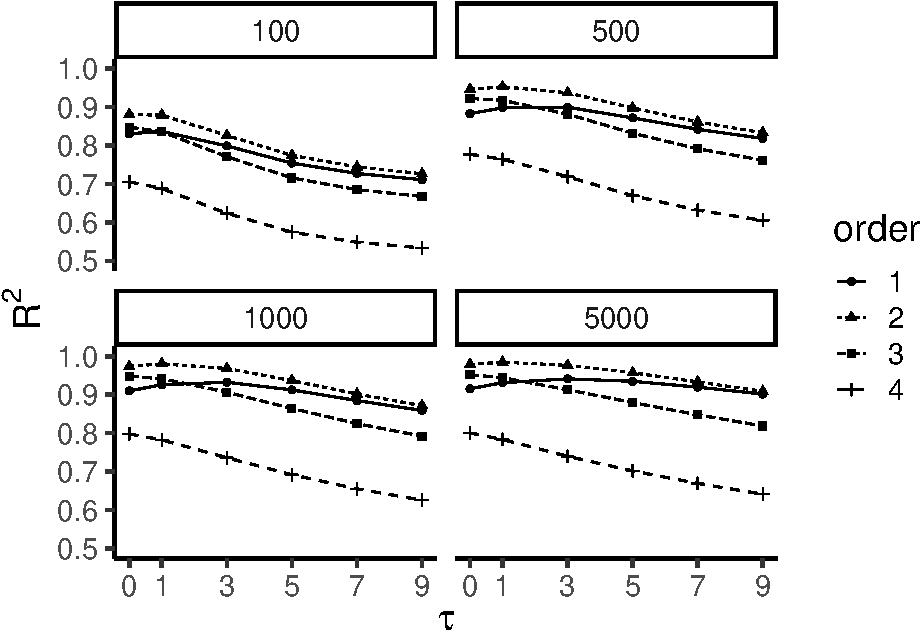
\includegraphics[width=\linewidth]{ITS_cogsci_files/figure-latex/ITSsimple-1.pdf}
\caption{\label{fig:ITSsimple}\(R^2\) values between ITS word-word similarity space (the resulting matrix of word to-word similarities using ITS semantic vectors), and the first to fourth order word-word similarity spaces derived from the artificial language (e.g., those shown in the bottom panel of Figure 1), as a function of training, and retrieval gradient ($\tau$)}
\end{figure}

ITS performed well in recovering the structure of the language, and \emph{was most sensitive to second-order similarity space}. Overall, ITS became more sensitive to all orders of similarity as training increased, and less sensitive as $\tau$ increased. Raising $\tau$ did increase relative sensitivity to the first order, but did so at the cost of losing sensitivity overall. Specifically, increasing the selectivity of the retrieval gradient limits the sampling of traces into the echo, resulting in noisier representations. The fact that ITS prioritizes the second order over the first is a flaw. The second order space is an overgeneralized version of the first, and blurs out the finer distinctions between word usage within the topic structures that generate the words. ITS relies on second order similarity (see discussion), so semantic vectors for topic-unique words become similar to words from overlapping topics, whereas they are not similar to those words in first order space. ITS glosses over these nuances.

\subsection{Simulation 2: ITS 2 encoding}

We next trained ITS 2 with \emph{weighted expectancy subtraction} at encoding on the same artificial language. We show that weighted expectancy subtraction causes ITS 2 to become more sensitive to first order word-word similarity than higher orders. In the simulations we vary the value of \(x\) (from .01 to .5) to subtract different amounts of the echo from the probe. The value of \(x\) causes systematic differences in ITS 2's sensitivity to higher order similarity structure. For brevity, we report results with \(\tau\) set to 1 (shown in figure \ref{fig:allsims}, left panel).

\begin{figure*}

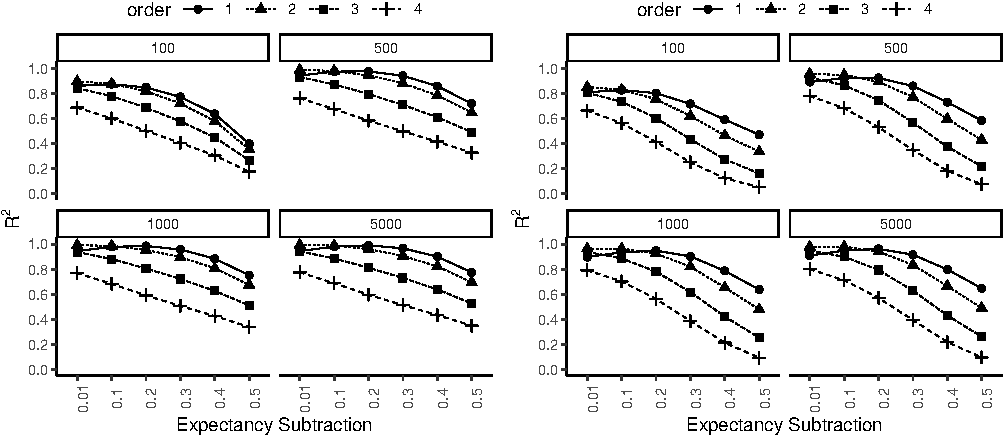
\includegraphics[width=\textwidth]{ITS_cogsci_files/figure-latex/allsims-1.pdf}

\caption{\(R^2\) values between ITS word-word similarity space and the first to fourth order word-word similarity spaces derived the artificial language as a function of training, and \emph{weighted expectancy subtraction}. The left panel shows ITS 2 with weighted expectancy subtraction during encoding, and the the right panel shows ITS 2 with weighted expectancy subtraction during retrieval.}\label{fig:allsims}
\end{figure*}

% \begin{figure}
% \centering
% 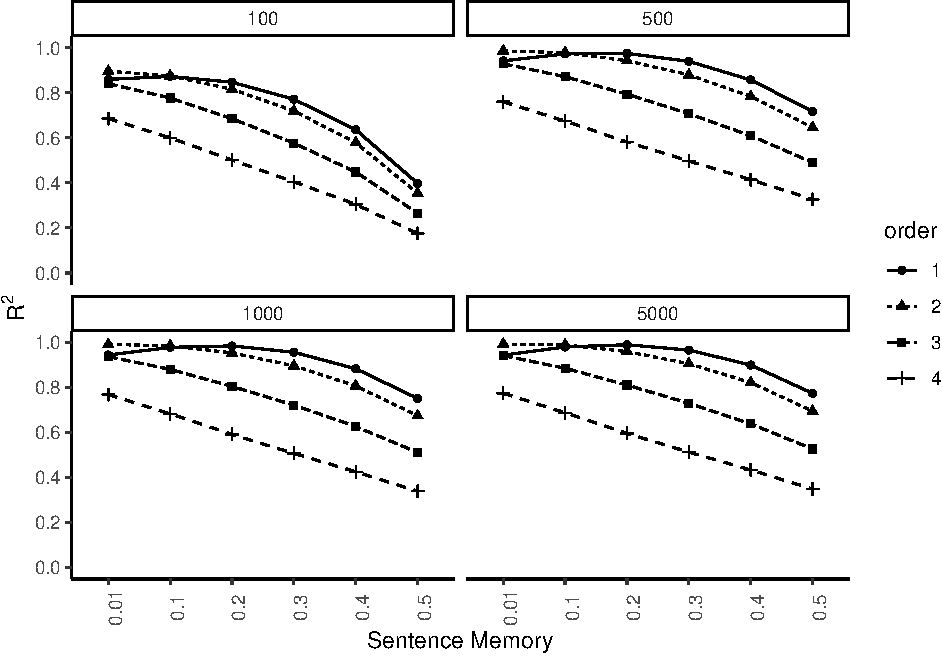
\includegraphics[width=\linewidth]{ITS_cogsci_files/figure-latex/ITSencodinglinear-1.pdf}
% \caption{\label{fig:ITSencodinglinear}\(R^2\) values between simple ITS word-word similarity space, and the first to fourth order word-word similarity spaces derived from the artificial language as a function of training, and \emph{weighted expectancy subtraction} at encoding. The retrieval gradient (tau) was set to 1.}
% \end{figure}

\emph{Weighted expectancy subtraction} at encoding modulated how ITS 2 recovered different orders of semantic similarity space, specifically allowing recovery of more veridical and nuanced word embeddings from the first-order similarity space. For example, when \(x=.01\), ITS 2 was most sensitive to second order similarity, but as \(x\) increased ITS 2 became most sensitive to first-order similarity. Increasing \(x\) further caused overall sensitivity to decline.

\subsection{Simulation 3: ITS 2 retrieval}

Here, we repeated the above simulation but applied \emph{weighted expectancy subtraction} with \emph{iterative retrieval} after training was complete (using standard ITS memory encoding). The results are shown in figure \ref{fig:allsims} (right panel).

% \begin{figure}
% \centering
% 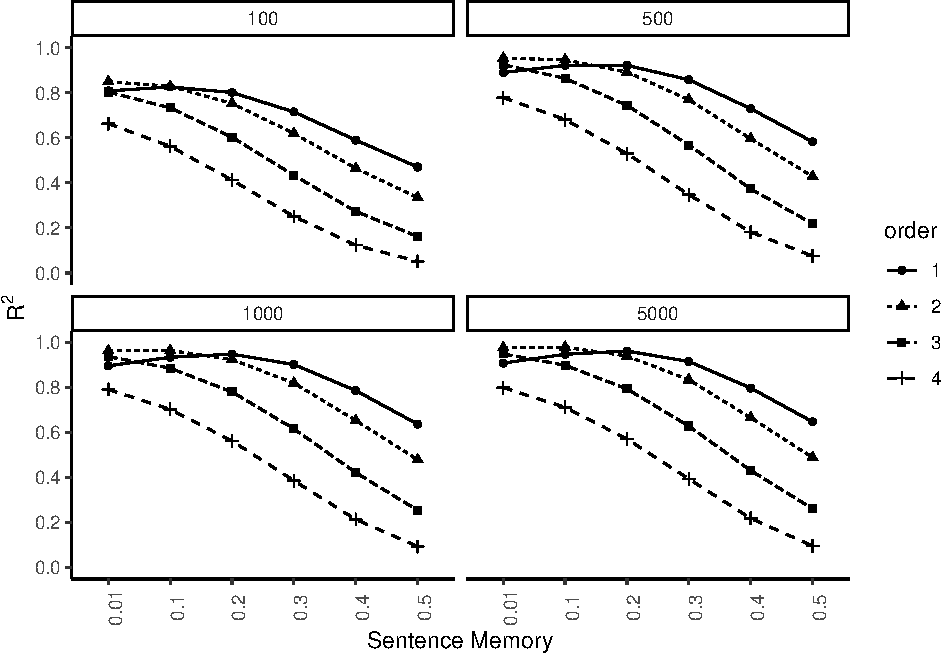
\includegraphics[width=\linewidth]{ITS_cogsci_files/figure-latex/ITSretrieval-1.pdf}
% \caption{\label{fig:ITSretrieval}\(R^2\) values between simple ITS word-word similarity space, and the first to fourth order word-word similarity spaces derived from the artificial language as a function of training, and \emph{weighted expectancy subtraction} at retrieval.}
% \end{figure}

Remarkably, ITS 2 does not need to make any assumptions about encoding to benefit from \emph{weighted expectancy subtraction}. The pattern of Simulation 3 is almost identical to that of Simulation 2. Specifically, ITS 2 becomes most sensitive to first-order word-word similarity structure as \(x\) is increased. Again, increasing \(x\) has diminishing returns.

\section{General Discussion}

We showed that ITS is most sensitive to second order semantic space, and that ITS 2 increases sensitivity to the more veridical first order space by processes of \emph{weighted expectancy subtraction} and \emph{iterative retrieval}.

It is instructive to consider how ITS and ITS 2 recover different orders of similarity space. First, consider how words become increasingly similar across orders of similarity space. In the first order, word similarity is determined by the topics they occur in. Word 6 is unique to topic one and only similar to words in topic one. In the second order, words become similar on the basis of their first-order similarity features. First-order features for word 6 contain positive similarity for topic one words 1 to 15. Some of these features (11 to 15) are shared by words from topic two, so word 6 becomes similar to topic two words in second order space. If topics are connected by overlapping words, then all words become increasingly similar across increasing orders of similarity, and the nth order similarity matrix becomes all ones.

Crucially, \emph{iterative retrieval} in ITS 2 is a process for traversing higher-order similarity space; and \emph{weighted expectancy subtraction} is a process for negotiating the relative contributions of higher-order similarity in the construction of semantic knowledge. To elaborate, we showed that standard ITS echoes are most sensitive to the second order. Echoes contain sentence memory, so an echo for a topic-unique word is immediately partially similar to echoes for words from neighboring topics, because their echoes share co-occurring words. Submitting an echo as a probe for iterative retrieval is a third order operation. The echo contains many words and the second echo collapses over memory for sentences that contain any of those words. This draws in sentences from additional topics, causing a given word to be more similar to words in more distant topics. Iterating to the extreme sweeps all sentences in memory into the echo, causing identical echoes for all words.

Simulation 3 showed that subtracting a portion of the second echo from the first allows ITS 2 to preferentially recover first order space. Our preceding discussion suggests ITS 2 performs a weighted subtraction of third from second order space, implying a similar result could be obtained analytically. We confirmed this directly from the language in the following way.

\begin{figure}
\centering
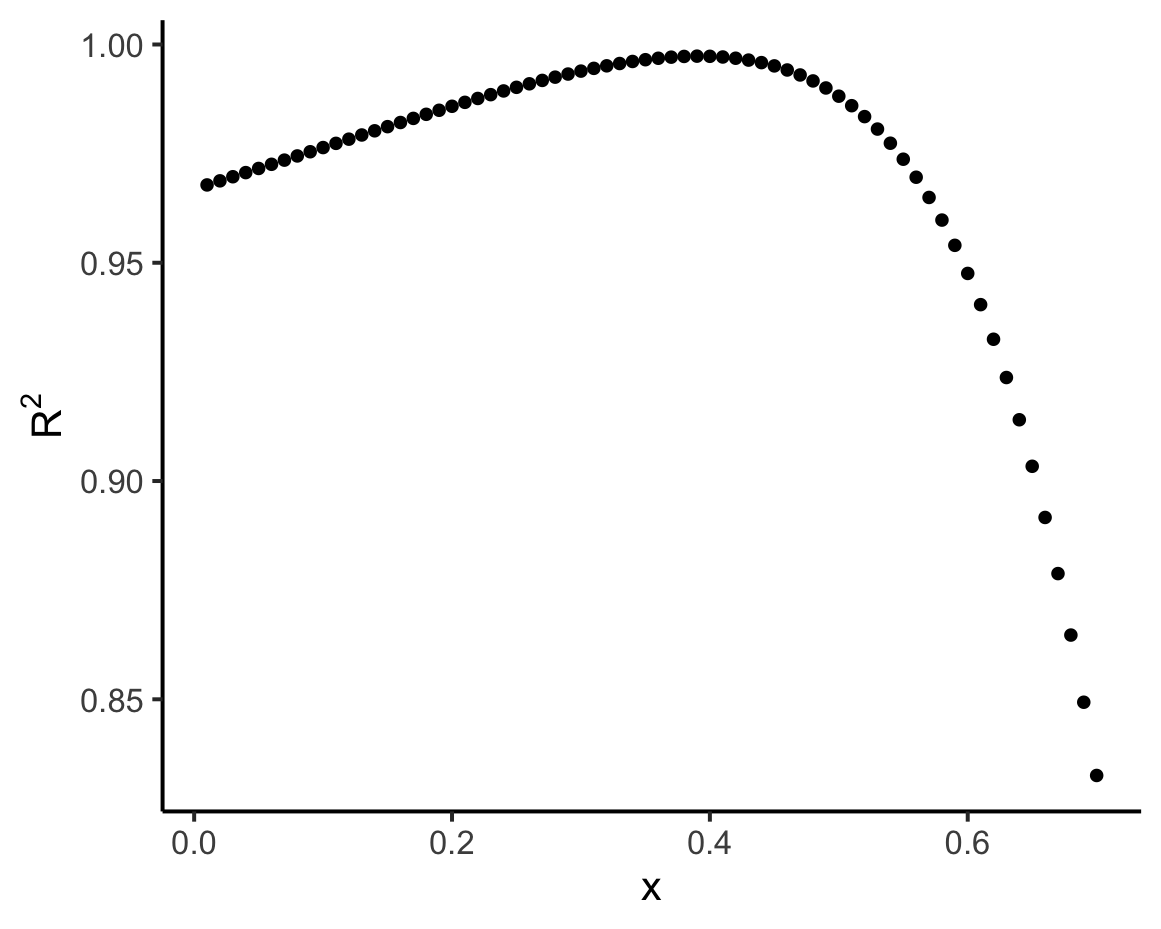
\includegraphics[width=\linewidth]{ITS_cogsci_files/figure-latex/recon.png}
\caption{\label{fig:firstRecon}\(R^2\) values between first-order word-word similarity and the weighted subtraction of third order space from second order space, as a function of $x$, the proportion of third order space subtracted from the second.}
\end{figure}

First, we computed the third and second order word-word similarity matrices directly from the language (as shown in bottom 2 and 3rd panel of Figure 1). Next, we attempted reconstruction of the first-order word-word similarity matrix by subtracting proportions, $x$, of the third order matrix from the second order matrix. For each value of $x$, we computed $R^2$ between the resulting matrix and the first order similarity matrix. The results are shown in Figure 4. The result is an inverse U function, with \(R^2\) approaching 1 at $x$ = .4. So it appears that, at least for this toy language, the particulars of word meaning in the first order, that are overgeneralized in the second and third orders, can actually be recovered by subtracting a weighted portion of the third order similarity space from the second. 

As a sidenote, computing second order similarity from a document term matrix  \cite{cribbinDiscoveringLatentTopical2011} can produce embeddings similar to those produced by singular value decomposition, as in LSA \cite{landauerSolutionPlatoProblem1997}. We speculate that subtracting a portion of the third order from the second may further improve the quality of those semantic representations.

More generally, count-based/vector-accumulation models like ITS rely exclusively on positive information from word co-occurrence, whereas neural embedding models like word2vec \cite{mikolovDistributedRepresentationsWords2013} exploit negative information by sub-sampling adversarial examples during training which may result in superior word embeddings \cite{manderaExplainingHumanPerformance2017a}. \citeauthor{johnsRoleNegativeInformation2019} \citeyear{johnsRoleNegativeInformation2019} developed analytic transformations for weighting word occurrence base rates that approximate gains from using negative information for improving word-embedding quality. We speculate that ITS 2 negotiates a similar merger of general expectations for word occurrence in higher order space with specific expectations from lower order space by \emph{iterative retrieval} and \emph{weighted expectancy subtraction}; and, may realize base-rate transforms through cognitive encoding and retrieval operations.

As a future direction we will apply ITS and ITS 2 to natural language and determine whether ITS 2 assumptions produce higher quality fits to human semantic judgments. At present, we offer ITS 2 as an intriguing account of how people may transform their semantic knowledge along general versus specific lines, by using 
\emph{iterative retrieval} to traverse higher order similarity space, and \emph{weighted expectancy subtraction} to control the specificity of retrieved semantic knowledge.

Finally, it is worth considering the psychological plausibility of the proposed mechanisms for controlling retrieval and construction of semantic knowledge. We suggest that although \emph{iterative retrieval} may not be commonly explored in the context of MINERVA modeling, on its face, we think that most people would recognize iterative retrieval as a natural part of their own thinking. For example, speaking subjectively, it is common to have one thought lead to another, as if the production of a first idea was used a cue to retrieve and the next one. Admittedly, the process of  \emph{weighted expectancy subtraction} is less obvious as a subjectively identifiable psychological process. However, expectancy subtraction, in the form of surprise or error-driven learning \cite{rescorlaTheoryPavlovianConditioning1972}, is a fundamental feature of most basic psychological learning processes. So, we remain intrigued about prospects for an integrated account of semantic knowledge that encompasses basic learning and memory processes.

%
%
% Using the identity matrix to represent words, and setting tau to 0, ITS memory becomes a simple document-term matrix, and the echo for any probe is the sum of document vectors that contain the probe word. Consider that in first order space, words that are unique to one topic (e.g., words 6-10 for topic one) are only similar to themselves, and have zero similarity to all other words. However, this changes in second order space.
%
% If we use an identity matrix to represent words, and set tau to 0, it becomes
%
% It is not surprising that ITS is most sensitive to second order similarity space. Co
%
% We now attempt to clarify analytic relationships between ITS semantic vectors and higher order similarity space
%
%
% Our simulation approach offered some insight into
%
% We have shown that simple ITS is most sensitive to the second order word-word similarity structure of the artificial language. We discussed how \emph{iterative retrieval} produces echoes that would become more sensitive to increasing orders of word-word similarity space. Simulation 3 showed that subtracting a portion of the second echo from the first cause ITS 2 to become more sensitive to first order word-word similarity. These relationship suggest that \emph{weighted expectancy subtraction} is a transform that can be applied directly to higher order similarity space, if that space is known.
%
% In our case, the nth-order word-word similarity space is completely determined by the topic-word probability matrix of the artificial language. As a result, we can determine whether subtraction of a higher-order similarity space from a lower order similarity produces similar results. We assume that ITS 2 is performing an operation similar to subtracting a proportion of third-order word-word similarity space from it's representation of second-order word-word similarity space, and this subtraction results in an echo most sensitive to first-order word-word similarity space. We now show this by subtracting weighted portions of third-order word-word similarity space from the second-order to arrive at the first-order, directly from the basis functions of the artificial language.

%
% instance theory
%
% In other cognitive domains like categorization and concept formation major debate about representation and process has unfolded between prototype theories and exemplar or instance-based theories. In general, exemplar theories unfairly outgun prototype theories because memory is allowed to preserve the examples that prototype theory averages over, thus exemplar theories can variously reconstruct prototypes or specific examples depending on retrieval conditions. For example, the instance-based memory model MINERVA 2 can retrieve prototype representations from the ganged retrieval of noisy exemplars, or single traces depending on
%
% We avoid declaring a winner, but point out that instance theories have had clear success in explaining a variety of cognitive phenomena by models that jointly articulate representational assumptions along with processing assumptions.
%
% Outside of distributional semantic models, proty
%
% , debate has centered on alternatives to prototype representation
%
%
%  prototype theories have often been replaced by more powerful exemplar or instance-based approaches.
%
% Additionally, just as a prototype can be similar to different meanings of a word, it can preserve some sensitivity to general and specific meaning (e.g., cat can be similar to lion and animal).
%
%
%
% But, these models also make simplifying assumptions about semantic representations that are problematic from the perspective of production, which we assume plays a role both in the construction and use of semantic knowledge.
%
% A major simplifying assumption from many representational models is the adoption of prototype representation.
%
%
% So, like people, prototype models posesses representations of semantic meaning sensitive to multiple levels of similarity; but perhaps unlike people, they do not allow
%
%
% In some sense prototype models are impressive because their representations do capture word meaning at multiple levels of similarity
%
%
% Nevertheless, the prototypical status of a word is despite the fact that word representations are stable, and unable to be repositioned for comparing semantic similarity at different levels,
%
% Critically, each semantic vector is a singular and canonical prototypical average of how a word co-occurs with other words in local contexts. The theoretical implication is that
%
%
% Although some aspects of general and specific meaning can be preserved in this space (e.g., cat can be similar to lion and animal), the models decline to assign a role for production flexibly construct semantic representations at different levels of specificity.
%
%  However, despite explaining how distributed knowledge of word co-occurence may form a basis for semantic representation, these models refrain from describing production processes likely involved in using and constructing semantic representations. Furthermore, semantic vectors for words are given singular and canonical prototype representations.
%
%  and words closer together in semantic space are
%
%
%  In the and words become more similar in meaning as they approach each other in semantic space.
%
%
%
%  Semantic meaning between words is computed in terms of the distance or angle between words in high-dimensional space.
%
%  The
%
%  Representation models
%
% Distributional models of semantics produce word embeddings sensitive to word co-occurrence structure in natural text. Word embeddings are more similar between words appearing in similar than different local contexts (sentences, paragraphs). The quality of word embeddings depends on their use. For applied purposes, word-embeddings could be used to train a classifier (e.g., for sentiment analysis) and quality assessed by classifier accuracy. For theoretical purposes, distributional models of semantic cognition are evaluated by fits to human performance in semantic tasks. Word embedding quality also depends on base rates of word occurrence. High frequency words can dominate semantic vectors, causing embeddings to become more similar and less indicative of nuanced meaning. Standard approaches to managing base rate information have questionable cognitive plausibility.
%
% Common base rate management strategies are stop word exclusion, transformation, and negative sub-sampling. Stop word exclusion is arbitrary and fails to account for included word base rates. Early models like LSA \cite{landauerSolutionPlatoProblem1997} used transformation. Word frequencies were log transformed and divided by their entropy across document contexts. The log transform compresses frequency counts, and the division by entropy weights words by the specificity of their occurrence in local contexts. Here, context-ubiquitous high-frequency words (high entropy) are weighted less strongly than context-specific words (low entropy). Neural network models like word2vec \cite{mikolovDistributedRepresentationsWords2013} use a process of sub-sampling adversarial examples during training. Here, network weights are modified by prediction error from positive and negative examples; and, negative examples are chosen randomly as a function of word frequency. Importantly, word2vec produces high-quality word embeddings that can explain more variance in human semantic judgments than other models \cite{manderaExplainingHumanPerformance2017a}, and these improvements have been attributed to the sub-sampling procedure. Relatedly, \citeauthor{johnsRoleNegativeInformation2019} \citeyear{johnsRoleNegativeInformation2019} created analytic transforms mimicking the base rate management effects of sub-sampling negative information that appear to improve the quality of word-embeddings in general.
%
% We are optimistic that distributional models hold insights for semantic cognition, but we question the cognitive plausibility of common strategies for managing base rate information. It is unlikely that people ignore stop words, unclear how people would weight word frequency knowledge by information theoretic transforms (or apply singular value decomposition), and doubtful that people employ negative sub-sampling when they encounter words. In our view, a satisfactory model should detail a cognitively plausible process for managing base rates in constructing semantic knowledge. We propose a cognitive solution for the ITS model that merges theoretical insights from traditions in memory and learning.



% \section{Acknowledgments}
%
% In the \textbf{initial submission}, please \textbf{do not include
%   acknowledgements}, to preserve anonymity.  In the \textbf{final submission},
% place acknowledgments (including funding information) in a section \textbf{at
% the end of the paper}.

\bibliographystyle{apacite}

\setlength{\bibleftmargin}{.125in}
\setlength{\bibindent}{-\bibleftmargin}

\bibliography{ITS}


\end{document}
